\section{Information Theory}

\begin{defn}
    \newterm{Information} is $I = -\log p(x)$
\end{defn}

\begin{defn}
    \newterm{Entropy} is the functional $H[p] = - \sum p(x) \log p(x) = E_p[log p(x)]$.
\end{defn}

\begin{defn}
    \newterm{Differential Entropy} is the functional $H[p] = - \int p(x) \log p(x) \dx$
\end{defn}

\begin{defn}
    \newterm{KL Divergence} (also known as \newterm{relative entropy} between a distribution $p$ and $q$ is
    
    \begin{align}
        \kldiv{p}{q} &= -\int p(x) \log q(x) + \int p(x) \log p(x) \dx  \\
        &= H[p, q] - H[p]
    \end{align}
\end{defn}

We can further simplify this as

\begin{align}
    \kldiv{p}{q} &= -\int p(x) \log q(x) + \int p(x) \log p(x) \dx  \\
    &= \int p(x) (\log p(x) - \log q(x)) \dx \\
    &= \int p(x) \log \frac{p(x)}{q(x)} \dx \\
    &= - \int p(x) \log \frac{q(x)}{p(x)} \dx.
\end{align}

Note that last two equations differ only in the minus sign, which flips the fraction.

\begin{thm}
The KL-divergence is invariant under parameter transformations \todo{proof}.
% https://en.wikipedia.org/wiki/Kullback%E2%80%93Leibler_divergence
\end{thm}

\begin{tcolorbox}
    Looking at the definition of entropy for each, we can view $\kldiv{p}{q}$ as sort of $H[q] - H[p]$, which would be
    
    \begin{align}
        H[q] - H[p] &= -\int q(x) \log q(x) \dx - \left( -\int p(x) \log p(x) \dx \right)
    \end{align}
    
    But since KL-divergence can be thought of as relative distance with respect to $p$, this turns into
    
    \begin{align}
        -\int p(x) \log q(x) \dx - \left( -\int p(x) \log p(x) \dx \right) = H[p, q] - H[p].
    \end{align}
\end{tcolorbox}

\subsection{Properties of the KL-divergence}

\begin{thm}
The KL-divergence is always positive.
\end{thm}

\begin{proof}
    % https://stats.stackexchange.com/questions/335197/why-kl-divergence-is-non-negative
    \begin{align}
        0 \leq \kldiv{p}{q} = - \int p(x) \log \frac{q(x)}{p(x)} \dx
    \end{align}
\end{proof}

\begin{thm}
$\kldiv{p}{q} \neq \kldiv{q}{p}$
\end{thm}


\begin{tcolorbox}
Explain KL-divergence as a relative distance. 

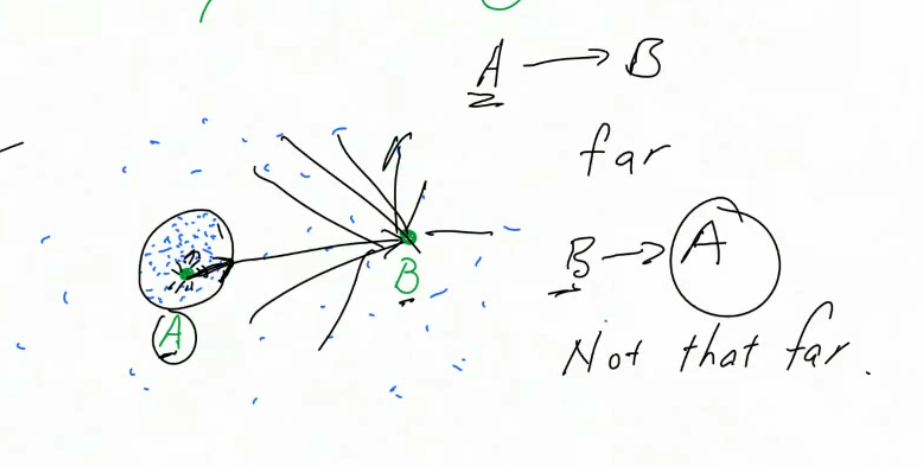
\includegraphics[width=0.7\textwidth]{img/kldivergence-relative}
\end{tcolorbox}



\subsection{Relationship between $\log p(x)$ and $D_{KL}$}

Let's say we have a distribution $p(z | x)$ which we don't know, and we want to use $q(z)$ to estimate it. We use the KL-divergence to measure the quality of the esimate, that is $\kldiv{q(z)}{p(z|x)}$.

\begin{align}
    \label{eq:kldiv}
    \kldiv{q(z)}{p(z|x)} = - \int q(z) \log \frac{p(z|x)}{q(z)} \dz
\end{align}

We know from conditional probability that

\begin{equation}
    \frac{p(x,z)}{p(x)} = p(x|z)
\end{equation}

and plugging that back into \ref{eq:kldiv} we get

\begin{align}
    \kldiv{q(z)}{p(z|x)} &= - \int q(z) \log \frac{p(z|x)}{q(z)} \dz \\
    &= - \int q(z) \log \left( \frac{p(x,z)}{p(x)}  \frac{1}{q(z)} \right) \dz \\
    &= - \int q(z) \left( \log \frac{p(x,z)}{q(z)} + \log \frac{1}{p(x)} \right) \dz \\
    &= - \int q(z) \log \frac{p(x,z)}{q(z)} \dz - \int q(z) \log \frac{1}{p(x)} \dz \\
    &= - \int q(z) \log \frac{p(x,z)}{q(z)} \dz + \int q(z) \log p(x) \dz \\
    &= - \int q(z) \log \frac{p(x,z)}{q(z)} \dz + \log p(x) \int q(z) \dz \\
    &= - \int q(z) \log \frac{p(x,z)}{q(z)} \dz + \log p(x)
\end{align}

and moving the first term to the left side of the equation gives us

\begin{equation}
    \kldiv{q(z)}{p(z|x)} + \int q(z) \log \frac{p(x,z)}{q(z)} \dz = \log p(x).
\end{equation}

We call the second quantity on the left the \newterm{variational lower bound} (also known as ELBO for \newterm{expected lower bound}) and we denote it as $\gL$. For clarity, let us denote $D_{KL} = \kldiv{q(z)}{p(z|x)}$ in the rest of this section.

\begin{equation}
    D_{KL} + \gL = \log p(x).
\end{equation}

Here we make a few observations. First of all, note that $\gL = -D_{KL}$ \todo{je tohle fakt pravda?}, which is always negative. The initial KL-divergence is always positive, and since $0 < p(x) < 1$ \todo{tohle ale neni nutne pravda pro density? pro diskretni to ale plati ... tzn domyslet continuous case} we get $\log ([0; 1])$ on the right, which is always negative.

\begin{equation}
    \underbrace{D_{KL}}_{\text{always +}} + \underbrace{\gL}_{\text{always -}} = \underbrace{\log p(x)}_{\text{always -}}
\end{equation}

Because we started with $p(z|x)$ we know $x$ is some fixed value which does not change as we optimize $q(z)$ to approximate it. This means the right side $\log p(x)$ is also fixed. As a result, changing $\gL$ will change the value of $D_{KL}$ which matches our intuition.

A key insight here is that increasing $\gL$ immediately decreases $D_{KL}$, because $\gL$ is negative, $D_{KL}$ is positive, and $\log p(x)$ does not change as $q(z)$ changes.

\subsection{Useful inequalities}

\begin{thm}[Log-sum inequality]
TODO
% https://en.wikipedia.org/wiki/Log_sum_inequality
\end{thm}

\begin{thm}[Gibbs' inequality]
TODO
% https://en.wikipedia.org/wiki/Gibbs%27_inequality
\end{thm}

\begin{thm}[Jensen inequality]
% https://en.wikipedia.org/wiki/Jensen's_inequality
\end{thm}
